\section{Ángulos}
\subsection{¿Qué es un ángulo?}

\begin{definition}
	Un \textbf{ángulo} se define como la abertura (o región del plano) 
	comprendida entre los semirectas que tienen un origen en común, 
	llamado \textit{vértice}
\end{definition}

\begin{figure}[hb]
	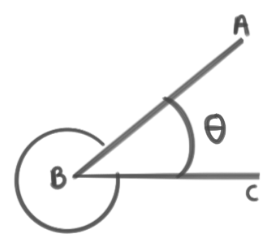
\includegraphics[width=0.40\textwidth]{angulo}
	\caption[Angulo]{Ángulo ABC. En donde:
	\begin{itemize}
		\item \textbf{B} es el vértice del ángulo
		\item $\pmb{\overline{BC}}$ es el lado inicial del ángulo
		\item $\pmb{\overline{BA}}$ es el lado final o terminal del ángulo
	\end{itemize} }
	\labfig{angulo}
\end{figure}

\marginnote[2mm]{$\pmb{\overline{BA}}$ se lee como el segmento BA}

\begin{itemize}
	\item De manera gráfica un ángulo se representa mediante un arco de 
	circunferencia.

	\item Es importante destacar que las dos semirectas siempre formarán 
	\textit{dos ángulos}:
	
	\begin{itemize}
		\item Un ángulo \textbf{interno} y
		\item Un ángulo \textbf{externo}
	\end{itemize}

	\item Por último, si juntamos (sumamos) el ángulo \textbf{interno} y 
	el \textbf{externo} obtendremos una vuelta, mejor conocida como 
	\textbf{revolución}

\end{itemize}

Otras consideraciones importantes para trabajar con ángulos son que:

\begin{itemize}
	\item La simbología para representar ángulos es variada, se sueleve usar: 
	$\pmb{\angle,\; \measuredangle}$, $\angle\; A$, $\hat{a}$
	\begin{itemize}
		\item También se suele utilizar la notación $\pmb{\angle ABC}$
		\item De la cual se debe entender que la letra de en medio representa el 
		vértice del ángulo al que se hace referencia.
	\end{itemize}
	\item Tamién es posible representar los ángulos con letras griegas,
	por ejemplo: $\pmb{\alpha,\; \beta,\; \gamma,\; ...}$
	%TODO:- Agregar más colores
	\item \textbf{Si el ángulo se mide en sentido \textit{contrario a las 
	manecillas del reloj}, entonces es \textit{positivo}}.
	\sidenote[][-6cm]{\textbf{Ángulo positivo}\\ 
	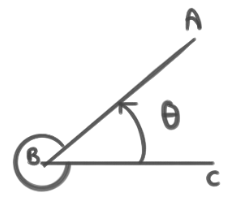
\includegraphics[width=3.5cm]{angpos}}
	\item \textbf{Si el ángulo se mide en sentido \textit{de las 
	manecillas del reloj}, entonces es \textit{negativo}}.
	\sidenote[][-2cm]{\textbf{Ángulo negativo}\\ 
	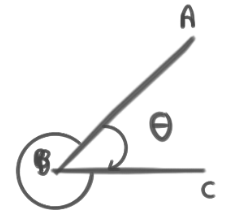
\includegraphics[width=3.5cm]{angneg}}
\end{itemize}

\subsection{Clasificación de ángulos}

\subsubsection{Primera clasificación}

Los ángulos pueden ser clasificados de acuerdo a su medida como se muestra en la
tabla \ref{clasifangulos}.

\begin{figure*}[h!]
% \begin{adjustbox}{max width=16.3cm}
\def\arraystretch{1.5}%  1 is the default, change whatever you need
\caption[Clasificación de ángulos]{Clasificación de ángulos. 
	Se toma como base su medida
}
%TODO:- Corregir referencia de la tabla.
\labtab{clasifangulos}
\label{clasifangulos}
\begin{tabular}{c | c | c }
	% \hline
	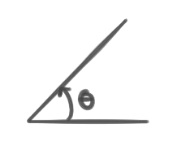
\includegraphics[width=4cm]{agudo} & 
	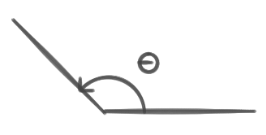
\includegraphics[width=4cm]{obtuso}  & 
	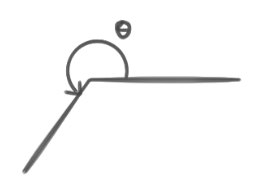
\includegraphics[width=4cm]{entrante} 
	\\ %\hline

	\textbf{Agudo} & 
	\textbf{Obtuso} & 
	\textbf{Entrante}                       
	\\ %\hline

	$0^\circ < \theta < 90^\circ$ &
	$90^\circ < \theta < 180^\circ$ &
	$180^\circ < \theta < 360^\circ$ 
	\\

	\parbox{4cm}{
		\begin{center}
			Mayores que $0^\circ$ y \\ Menores que $90^\circ$
		\end{center} 
	} & 
	\parbox{4cm}{
		\begin{center}
			Mayores que $90^\circ$ y \\ Menores que $180^\circ$
		\end{center} 
	} & 
	\parbox{4cm}{
		\begin{center}
			Mayores que $180^\circ$ y \\ Menores que $360^\circ$
		\end{center} 
	}                                 
	\\ \hline

	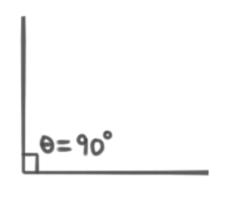
\includegraphics[width=4cm]{recto} & 
	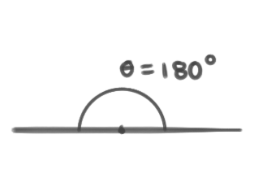
\includegraphics[width=4cm]{llano} & 
	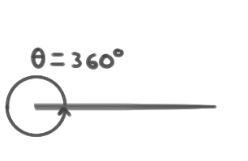
\includegraphics[width=4cm]{perigonal} 
	\\ %\hline
	\textbf{Recto} & 
	\textbf{Llano}  & 
	\textbf{Perigonal o de vuelta completa} 
		\\ %\hline

	$\theta = 90^\circ$ &
	$\theta = 180^\circ$ &
	$\theta = 360^\circ$ 
	\\

	\parbox{4cm}{
		\begin{center}
			Exactamente $90^\circ$
		\end{center} 
	} & 
	\parbox{4cm}{
		\begin{center}
			Exactamente $180^\circ$
		\end{center} 
	} & 
	\parbox{4cm}{
		\begin{center}
			Exactamente $360^\circ$
		\end{center} 
	}                                 
	% \\ \hline
\end{tabular}
% \end{adjustbox}
\end{figure*}

\subsubsection{Segunda clasificación}

La segunda clasificación de ángulos hace uso del concepto de ángulo 
\textit{recto}, \textit{llano} y \textit{perigonal}. Dicha clasificación se 
da siempre para dos o más ángulos a través del concepto de completariedad y 
sumplementaridad como se ve a continuación.


\begin{figure*}[h!]
% \begin{adjustbox}{max width=16.3cm}
\def\arraystretch{1.5}%  1 is the default, change whatever you need
\caption[Clasificación de ángulos]{Segunda clasificación de ángulos. 
	Se toma como base su la completariedad o sumplementaridad entre ellos.
}
%TODO:- Corregir referencia de la tabla.
\labtab{clasifangulosdos}
\label{clasifangulosdos}
\begin{tabular}{c | c | c }
	% \hline
	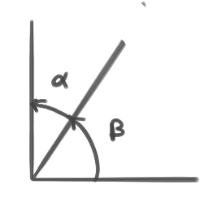
\includegraphics[width=4cm]{complementario} & 
	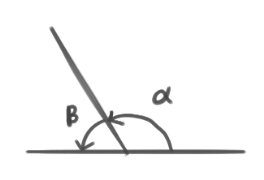
\includegraphics[width=4cm]{suplementario}  & 
	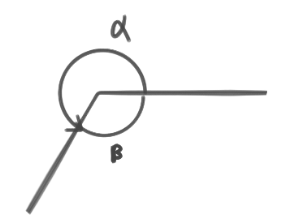
\includegraphics[width=4cm]{conjugado} 
	\\ %\hline

	\textbf{Ángulos complementarios} & 
	\textbf{Ángulos suplementarios} & 
	\textbf{Ángulos conjugados}                       
	\\ %\hline

	$\angle \alpha + \angle \beta= 90^\circ$ &
	$\angle \alpha + \angle \beta= 180^\circ$ &
	$\angle \alpha + \angle \beta= 360^\circ$ 
	\\

	\parbox{4cm}{
		\begin{center}
			La suma de los ángulos tiene que dar exactamente $90^\circ$
		\end{center} 
	} & 
	\parbox{4cm}{
		\begin{center}
			La suma de los ángulos tiene que dar exactamente $180^\circ$
		\end{center} 
	} & 
	\parbox{4cm}{
		\begin{center}
			La suma de los ángulos tiene que dar exactamente $360^\circ$
		\end{center} 
	}                                 

\end{tabular}
% \end{adjustbox}
\end{figure*}

%TODO:- Agregar ejemplos
\begin{figure*}[h!]
 \begin{kaoexercises}
	Hallar el valor de todos los ángulos en las siguientes figuras
  \begin{multicols}{3}
		\begin{enumerate}[itemsep=2pt,parsep=2pt]
			% 1
			\item \textbf{}\\
			\begin{tikzpicture}[scale=0.8]
  \draw
  (60:3) coordinate (c) node[right=2mm,above] {$C$} -- 
  (0,0) coordinate (o) node[left] {$O$} -- 
  (0,3) coordinate (b) node[above ] {$B$}
  pic["\rotatebox{45}{$6x-3^\circ$}",draw=orange,->,angle eccentricity=1.5,angle radius=1.5cm] 
    {angle=c--o--b};
  \draw (o) -- (3,0) coordinate (a) node[right] {$A$};
  \pic["$2x+5^\circ$",draw=orange,->,angle eccentricity=1.7,angle radius=1cm] 
  {angle=a--o--c};
\end{tikzpicture}
			
			% 2
			\item \textbf{}\\
			\begin{tikzpicture}[scale=0.8]
  \draw
  (60:3) coordinate (c) node[right=2mm,above] {$C$} -- 
  (0,0) coordinate (o) node[left] {$O$} -- 
  (0,3) coordinate (b) node[above ] {$B$}
  pic["\rotatebox{45}{$6x-3^\circ$}",draw=orange,->,angle eccentricity=1.5,angle radius=1.5cm] 
    {angle=c--o--b};
  \draw (o) -- (3,0) coordinate (a) node[right] {$A$};
  \pic["$2x+5^\circ$",draw=orange,->,angle eccentricity=1.7,angle radius=1cm] 
  {angle=a--o--c};
\end{tikzpicture}
			
			% 3
			\item \textbf{}\\
			\begin{tikzpicture}[scale=0.6]
  \coordinate (o) at (0,0);
  \coordinate (a) at (3,0);
  \coordinate (b) at (60:-3);
  \draw (o) -- (a) node [right] {$A$};
  \draw (o) -- (b) node [below]{$B$};
  \pic["$3(2x-1^\circ)+21^\circ$",draw=orange,->,angle eccentricity=1.5,angle radius=0.8cm]
    {angle=a--o--b};
  \pic["$5(3x-2^\circ)+1^\circ$",draw=blue,->,angle eccentricity=1.5,angle radius=1cm]
    {angle=b--o--a};
\end{tikzpicture}

			% 4
			\item \textbf{} \\
			\begin{tikzpicture}[scale=0.6]
  \draw
  (30:3) coordinate (c) node[right,above=1mm] {$C$} -- 
  (0,0) coordinate (o) node[below] {$O$} -- 
  (120:3) coordinate (d) node[above ] {$D$}
  pic["$90^\circ$",draw=blue,->,angle eccentricity=1.6,angle radius=5mm] 
    {angle=c--o--d};
  \draw (o) -- (3,0) coordinate (a) node[right] {$A$};
  \draw (o) -- (-3,0) coordinate (b) node[left] {$B$};
  \pic["$\dfrac{-x+3^\circ}{6}$",draw=orange,->,angle eccentricity=2.4,angle radius=1cm] 
    {angle=a--o--c};
  \pic["$\dfrac{2x-3^\circ}{4}$",draw=orange,->,angle eccentricity=1.6,angle radius=1cm] 
    {angle=d--o--b};
\end{tikzpicture}	
			\columnbreak%

			% 5
			\item \textbf{} \\
			\begin{tikzpicture}[scale=0.6]
  \draw
  (30:3) coordinate (c) node[right] {$C$} -- 
  (0,0) coordinate (o) node[below] {$O$} -- 
  (120:3) coordinate (d) node[above ] {$D$}
  pic["$5x-15^\circ$",draw=blue,->,angle eccentricity=2.1,angle radius=5mm] 
    {angle=c--o--d};
  \draw (o) -- (3,0) coordinate (a) node[right] {$A$};
  \draw (o) -- (-3,0) coordinate (b) node[left] {$B$};
  \pic["$7x-32^\circ$",draw=orange,->,angle eccentricity=2.1,angle radius=1cm] 
    {angle=a--o--c};
  \pic["$20^\circ-3x$",draw=orange,->,angle eccentricity=1.9,angle radius=1cm] 
    {angle=d--o--b};
\end{tikzpicture}

			% 6
			\item \textbf{}\\	
			\begin{tikzpicture}[scale=0.6]
  \draw
  (0,0) coordinate (o) node[below] {$O$} -- 
  (160:3) coordinate (d) node[above ] {$D$}
  pic["$4x-10^\circ$",draw=blue,->,angle eccentricity=1.5,angle radius=5mm] 
    {angle=a--o--d};
  \draw (o) -- (3,0) coordinate (a) node[right] {$A$};
  \draw (o) -- (-3,0) coordinate (b) node[left] {$B$};
  \pic["$x+15^\circ$",draw=orange,->,angle eccentricity=1.9,angle radius=1cm] 
    {angle=d--o--b};
\end{tikzpicture}	

			% 7
			\item \textbf{} \\
			\begin{tikzpicture}[scale=0.6]
  \draw
  (30:3) coordinate (c) node[right] {$C$} -- 
  (0,0) coordinate (o) node[below] {$O$} -- 
  (150:3) coordinate (d) node[above ] {$D$}
  pic["$2x-5^\circ$",draw=blue,->,angle eccentricity=1.5,angle radius=5mm] 
    {angle=c--o--d};
  \draw (o) -- (3,0) coordinate (a) node[right] {$A$};
  \draw (o) -- (-3,0) coordinate (b) node[left] {$B$};
  \pic["$x+45^\circ$",draw=orange,->,angle eccentricity=1.9,angle radius=1cm] 
    {angle=a--o--c};
  \pic["$3x-10^\circ$",draw=orange,->,angle eccentricity=1.9,angle radius=1cm] 
    {angle=d--o--b};
\end{tikzpicture}	
			\columnbreak%

			% 8
			\item \textbf{}\\
			\begin{tikzpicture}[scale=0.8]
  \draw
  (3,0) coordinate (a) node[right] {$A$} --
  (0,0) coordinate (o) node[left,above] {$O$} --
  (0,-3) coordinate (b) node[below] {$B$};
  \draw (o) -- (-20:3) coordinate (c) node[right] {$C$};
  \draw (o) -- (-50:3) coordinate (d) node[right] {$D$};
  \pic["$x$",draw=orange,->,angle eccentricity=1.7,angle radius=1cm] 
    {angle=c--o--a};
  \pic["$2x$",draw=orange,->,angle eccentricity=1.7,angle radius=1cm] 
    {angle=d--o--c};
  \pic["$3x$",draw=orange,->,angle eccentricity=1.7,angle radius=1cm] 
    {angle=b--o--d};
\end{tikzpicture}

			% 9
			\item \textbf{}\\
			\begin{tikzpicture}[scale=0.6]
  \coordinate (o) at (0,0);
  \coordinate (a) at (3,0);
  \coordinate (b) at (300:3);
  \draw (o) -- (a) node [right] {$A$};
  \draw (o) -- (b) node [below]{$B$};
  \pic["$12x+10^\circ$",draw=orange,->,angle eccentricity=1.8,angle radius=0.8cm]
    {angle=a--o--b};
  \pic["$x+25^\circ$",draw=blue,->,angle eccentricity=1.8,angle radius=1cm]
    {angle=b--o--a};
\end{tikzpicture}	

			% 10
			\item \textbf{} \\
			\begin{tikzpicture}[scale=0.6]
  \draw
  (30:-3) coordinate (c) node[below=1mm] {$C$} -- 
  (0,0) coordinate (o) node[below] {$O$} -- 
  (150:-3) coordinate (d) node[below=1mm ] {$D$}
  pic["$\dfrac{x}{2}$",draw=blue,->,angle eccentricity=1.9,angle radius=5mm] 
    {angle=c--o--d};
  \draw (o) -- (3,0) coordinate (a) node[right] {$A$};
  \draw (o) -- (-3,0) coordinate (b) node[left] {$B$};
  \pic["$\dfrac{x}{6}$",draw=orange,->,angle eccentricity=1.7,angle radius=1cm] 
    {angle=b--o--c};
  \pic["$\dfrac{x}{3}$",draw=orange,->,angle eccentricity=1.7,angle radius=1cm] 
    {angle=d--o--a};
\end{tikzpicture}				

		\end{enumerate}
  \end{multicols}
\end{kaoexercises}
\end{figure*}

\subsection{Sistema de medición de ángulos}

Para expresar la medida de lo ángulos contamos con dos sistemas de medición.

\subsubsection{Sistema sexagesimal}

El sistema sexagesimal es un sistema de numeración de base 60 que se usaba en 
la antigüedad para medir tiempos (lo que ahora conocemos como horas, minutos y
segundos). Además, tiene la ventaja de tener muchos divisores por lo que 
hacer proporciones (comparaciones) entre cantidades, era relativamente sencillo.
En consecuencia, también fue utilzado para medir ángulos, partiendo de la idea 
de relacionarlo con el tiempo.

Así mismo, a la idea de relacionar la medida de los ángulos con el tiempo se le 
suma el hecho de que la circunferencia se divide en 360 partes, llamadas 
\textbf{grados} \sidenote[][-2.5cm]{Se representa con el símbolo $\circ$, por ejemplo,
$45^\circ$}.
\begin{itemize}
	\item El grado se parte en 60 partes llamadas \textbf{minutos}
	\sidenote[][-2.3cm]{Los minutos se representan con un apostrófe ('), por ejemplo,
	$45'$, se lee 45 minutos} 
	y
	\item El minuto se parte en 60 partes llamadas \textbf{segundos}
	\sidenote[][-1.6cm]{Los segundos se representan con dos apostrófes (''), por ejemplo,
	$27'$, se lee 27 segundos}.
\end{itemize}

\marginnote[-5mm]{En el sistema sexagesimal podemos tener la medida del ángulo
como una combinación de grados, minutos y segundos. 
Por ejemplo $34^\circ\; 27'\; 45''$. 
Lo anterior se lee como: ``34 grados, 27 minutos, 45 segundos''}

De esta manera surgen las siguientes equivalencias:

\begin{equation*}
\boxed{
\begin{array}{rcl}	
		1\; rev &=& 360^\circ \\
		1^\circ &=& 60\;' \\
		1\;' &=& 60\;'' 
	\end{array}
}
\end{equation*}

\subsubsection{Conversiones entre grados, minutos y segundos}
Para hacer la conversión de grados a minutos o de minutos a segundos basta con 
relacionarlos mediante una regla de tres. Sin embargo el esquema (REF) ilustra
una forma más fácil. 

\begin{figure}[hb]
	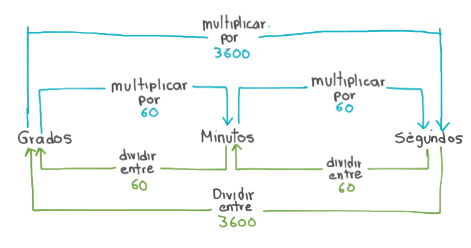
\includegraphics[width=\textwidth]{conversiongms}
	\caption[conversiongms]{Conversión entre grados, minutos y segundos.}
	\labfig{conversiongms}
\end{figure}

Veamos algunos ejemplos.

\begin{example}
	Convertir $\pmb{30^\circ\; 27'\; 38''}$ a Grados. \\
	\begin{enumerate}
		\item El primer paso consiste en transformar los minutos a grados. 
		Para ello:
		\begin{equation*}
			\dfrac{27'}{60} = 0.45^\circ
		\end{equation*}

		\item Luego, debemos de pasar los segundos a grados. Para ello: 
		\begin{equation*}
			\dfrac{38'}{3600} = 0.0105^\circ
		\end{equation*}

		\item Por último, como todas las cantidades están en la misma unidad, solo 
		queda sumarlas.
		\begin{align*}
			30^\circ\; 27'\; 38'' &= 30^\circ\; +\; 0.45^\circ\; +\; 0.0105^\circ \\
			\Aboxed{\pmb{30^\circ\; 27'\; 38''} &= 30.4605^\circ}
		\end{align*}

	\end{enumerate}
\end{example}

\begin{example}
	Convertir $\pmb{62.972^\circ}$ a grados y minutos
	\begin{enumerate}
		\item Lo primero que tenemos que hacer es descomponer $62.972^\circ$ en la 
		parte entera y la parte decimal. \\
		La parte entera ya se encuentra en grados por lo cual no hay nada más que 
		hacer.

		\item La parte decimal ($0.972^\circ$) la podemos transformar a minutos.
		Para ello, como lo indica el esquema \reffig{conversiongms}, debemos 
		\textbf{multiplicar por 60}
		\begin{equation*}
			0.972^\circ \times 60 = 58.32' 
		\end{equation*}

		\item Por último, se unen los grados y los minutos, de manera que nos queda 
		como: 
		\begin{equation*}
			\boxed{\pmb{62.972^\circ} = 62^\circ\; 58.32'}
		\end{equation*}
	\end{enumerate}
\end{example}

\begin{example}
	¿Qué pasa si nos piden convertir la cantidad anterior ($\pmb{62.972^\circ}$) a
	grados, minutos y segundos?
	\begin{enumerate}
		\item Debemos pasar la parte decimal ($.972^\circ$) a minutos.\\
		Lo cual da como resultado: $58.32'$.

		\item Ahora, la parte decimal de lo minutos ($0.32'$) debemos pasarla a 
		segundos. Para ello \textbf{multiplicamos por 60}:
		\begin{equation*}
			0.32 \times\ 60 = 19.2''
		\end{equation*}

		\item Por último, se unen los grados, minutos y segundos de la siguiente 
		forma:
		\begin{equation*}
			\boxed{\pmb{62.972^\circ} = 62^\circ\; 58'\; 19.2''}
		\end{equation*}
	\end{enumerate}
\end{example}

\begin{figure*}[h!]
 \begin{kaoexercises}
 Convierte los siguientes ángulos a \textit{solo} grados
 \begin{multicols}{4}
		\begin{enumerate}
		\setlength\itemsep{4mm}
		\item $40^\circ 10' 15''$
		\item $61^\circ 42' 21''$
		\item $1^\circ 2' 3''$
		\item $73^\circ 40' 40''$
		\item $9^\circ 9' 9''$
		\item $98^\circ 22' 45''$
		\item $23^\circ 24' 25''$
		\item $320^\circ 20' 17''$
		\item $322^\circ 50' 59''$
		\item $9^\circ 2' 1''$
	\end{enumerate}
 \end{multicols}

 Convierte los siguientes ángulos a su equivalente en grados, minutos y segundos.
 \begin{multicols}{4}
		\begin{enumerate}
		\setlength\itemsep{4mm}
		\item $40.32^\circ$
		\item $61.24^\circ$
		\item $18.255^\circ$
		\item $29.411^\circ$
		\item $19.99^\circ$
		\item $44.01^\circ$
		\item $32.123^\circ$
		\item $34.98^\circ$
		\item $32.29^\circ$
		\item $769^\circ$
	\end{enumerate}
 \end{multicols}

 \end{kaoexercises}
\end{figure*}

\subsubsection{Operaciones con ángulos}

Al igual que con los números arábicos, se pueden realizar las operaciones 
básicas con los ángulos en el sistema sexagesimal. A continuación veremos 
ejemplos de cómo realizar la suma, resta, multiplicación y división.\\

%TODO:- Revisar explicacion
Para realizar dichas operaciones basta con recordar dos cosas:
\begin{itemize}
	\item ``Peras con peras, manzanas con manzanas'', es decir, se deben operar
	grados con grados, minutos con minutos y segundos con segundos.

	\item Normalmente estamos acostumbrados a realizar operaciones en un sistema 
	decimal, es decir, base 10, pero, ¿Cómo realizariamos operaciones en un 
	sistema sexagesimal (base 60)?
	\begin{itemize}
		\item Analicemos que pasa en una suma en sistema decimal\\
		\begin{center}
			\begin{tabular}{c c c c}
				& \textcolor{red}{\pmb{1}}  & \textcolor{blue}{\pmb{1}} & \\
				& 4 & 3 & 4 \\
			+ &   & 9 & 8 \\
			\hline
				& 5 & 3 & 2 \\
			\end{tabular}
		\end{center}

		\begin{itemize}
			\item El máximo número que podemos poner es $9$ (el número anterior 
			a la base).
			\item Si el resultado de la suma de los primeros términos es mayor a $9$
			entonces solo se pone la unidad y la decena se pasa a la siguiente 
			posición.\\
			De esta manera, $4 + 8 = 12$, por lo tanto se pone el $2$ y el $1$ que
			representa las decinas se pasa a la siguiente posición.\\
			Este proceso se repite hasta que las se hayan recorrido todas las 
			posiciones de izquierda a derecha.
		\end{itemize}

		\item Ahora, intentemos realizar una operación en una \textbf{pseudo-base}
		\sidenote{Para que realmente fuera base 60 se necesitan 60 símbolos
		completamente distintos, cada uno representando una posición en la recta 
		númerica.\\ Por ejemplo un sistema base 2 solo tiene dos símbolos: $0$ y $1$
		} 60.

		\begin{center}
			\begin{tabular}{c c c c}
					& 40 & 38 & 12 \\
				+ &   & 49 & 47 \\
				\hline
			\end{tabular}
		\end{center}

		\begin{itemize}
			\item Debemos resolver de izquierda a derecha como en la suma con numeros 
			decimales
			\item El máximo número que podemos poner es 59 (uno antes que la base)
			\item Por lo tanto, $12 + 47 = \textcolor{orange}{59}$
			\begin{center}
				\begin{tabular}{c c c c}
						& 40 & 38 & 12 \\
					+ &   & 49 & 47 \\
					\hline
					& 		&    & \textcolor{orange}{59}
				\end{tabular}
			\end{center}

			\item Repetimos el mismo proceso para la siguiente posición: $38 + 49=87$,
			sin embargo, $87$ se puede expresar como $\textcolor{blue}{60} + 
			\textcolor{orange}{37}$. Por lo tanto podemos hacer lo siguiente:
			\begin{center}
				\begin{tabular}{c c c c}
						&\textcolor{blue}{60} & & \\
						& 40 & 38 & 12 \\
					+ &   & 49 & 47 \\
					\hline
					& 		& \textcolor{orange}{37}   & 59
				\end{tabular}
			\end{center}

			\item Una vez más hacemos lo mismo para $\textcolor{orange}{60} + 
			\textcolor{blue}{40} = 100$. Sin embargo no podemos escribir $100$ por lo 
			que dejamos los mismo números, por lo tanto queda como:
			\begin{center}
				\begin{tabular}{c c c c c}
						&\textcolor{blue}{60}& & & \\
						&& 40 & 38 & 12 \\
					+ &&   & 49 & 47 \\
					\hline
					& & \textcolor{orange}{40}		& 37   & 59
				\end{tabular}
			\end{center}

			\item Como 60 no tiene con quién sumarse simplemente lo 
			descomponemos como $\textcolor{orange}{59} + \textcolor{orange}{1}$, 
			porque el máximo número que podemos colocar
			es $59$. 
			\begin{center}
				\begin{tabular}{c c c c c c}
						&\textcolor{blue}{1}&& & & \\
						&&& 40 & 38 & 12 \\
					+ &&&   & 49 & 47 \\
					\hline
					&&\textcolor{orange}{59} & 40		& 37   & 59
				\end{tabular}
			\end{center}

			\item Por último, cómo $1$ no tiene con quién operarse simplemente lo 
			bajamos.
			\begin{center}
				\begin{tabular}{c c c c c c}
						&&& & & \\
						&&& 40 & 38 & 12 \\
					+ &&&   & 49 & 47 \\
					\hline
					&1&59 & 40		& 37   & 59
				\end{tabular}
			\end{center}
		\end{itemize}
	\end{itemize}

	\item Realizar operaciones con ángulos es más sencillo que el ejemplo 
	anterior debido a que tenemos el concepto de grado, minuto y segundo y sus 
	correspondentes equivalencias.
\end{itemize}

Veamos un ejemplo de cada operación:
\paragraph{Suma}

\begin{example}
	Realizar la siguiente operación:
		$39^\circ\; 48'\; 54'' + 18^\circ\; 23'\; 49'' $
	\begin{itemize}
		\item El primer paso es sumar los segundos. $54'' + 49'' = 103$. $103$ puede 
		ser reescrito como $\textcolor{blue}{60''} + \textcolor{orange}{43''}$. \\
		Además, $\textcolor{blue}{60''} = \textcolor{blue}{1'}$.
		\begin{center}
			\begin{tabular}{ c c c c}
					& & $\textcolor{blue}{1'}$ & \\
					& $39^\circ$ & $48'$ & $54''$ \\
				+ & $18^\circ$  & $23'$ & $49''$ \\
				\hline
				&  &   & $\textcolor{orange}{43''}$
			\end{tabular}
		\end{center}		

		\item Se repite el mismo proceso de tal manera que: $1' +'48' + 23' = 72'$.
		$72' = \textcolor{blue}{1^\circ} + \textcolor{orange}{12'}$
		\begin{center}
			\begin{tabular}{ c c c c}
					& $\textcolor{blue}{1^\circ}$ & $\textcolor{gray}{1'}$ & \\
					& $39^\circ$ & $48'$ & $54''$ \\
				+ & $18^\circ$  & $23'$ & $49''$ \\
				\hline
				&  & $\textcolor{orange}{12'}$   &$43''$
			\end{tabular}
		\end{center}	

		\item Finalmente, para los grados no es necesario pensar en términos de base 
		60, por lo que simplemente se suman sin importar que el valor sea mayor a 
		59.
		\begin{center}
			\begin{tabular}{ c c c c}
					& $39^\circ$ & $48'$ & $54''$ \\
				+ & $18^\circ$  & $23'$ & $49''$ \\
				\hline
				& $\textcolor{orange}{58^\circ}$ & $12'$   &$43''$
			\end{tabular}
		\end{center}	
	\end{itemize}
\end{example}

\paragraph{Resta}
La operación de resta o diferencia se realiza igual que en el sistema decimal y 
también se utiliza la clásica expresión de ``pedir prestado al número del lado 
izquierdo''.
\begin{example}
	Realizar la siguiente operación:
	$39^\circ\; 18'\; 34'' - 18^\circ\; 23'\; 49'' $
	\begin{itemize}
		\item Cómo $49''$ (sustraendo) es mayor que el $34''$ (minuendo) debemos
		``pedir préstamo'' al número de al lado. En este caso a \textit{18'}.\\
		Por lo que $18'$ se convierte el $17'$ y a $34''$ se le suma $1'$ o lo que 
		es lo mismo, $60''$, es decir:
		
		\begin{center}
			\begin{tabular}{ c c c c}
					& $39^\circ$ & 
					$\cancelto{\textcolor{orange}{17'}}{18'}$ & 
					$\cancelto{\textcolor{orange}{60'' + 34''}}{34''}$ \\
				- & $18^\circ$  & $23'$ & $49''$ \\
				\hline
				% &  &   & $\textcolor{orange}{43''}$
			\end{tabular}
		\end{center}	

	\item Reescribiendo en limpio y resolviendo la primera operación, nos queda 
	como:
	\begin{center}
		\begin{tabular}{ c c c c}
				& $39^\circ$ & 
				$17'$ & 
				$\textcolor{gray}{94''}$ \\
			- & $18^\circ$  & $23'$ & $49''$ \\
			\hline
			&  &   & $\textcolor{orange}{45''}$
		\end{tabular}
	\end{center}

	\item Se realiza el mismo proceso para $17'$ y $23'$:
	\begin{center}
		\begin{tabular}{ c c c c}
				& $\cancelto{\textcolor{orange}{38^\circ}}{39^\circ}$ & 
				$\cancelto{\textcolor{orange}{60' + 17'}}{17'}$ & 
				$34''$ \\
			- & $18^\circ$  & $23'$ & $49''$ \\
			\hline
			&  &   & $45''$
		\end{tabular}
	\end{center}	

	\item Como último paso se resuelve la resta entre minutos y se realiza 
	la operación con los grados, sin importar si el resultado queda como positivo 
	o negativo.
	\begin{center}
		\begin{tabular}{ c c c c}
				& $\textcolor{gray}{38^\circ}$ & 
				$\textcolor{gray}{77}'$ & 
				$34''$ \\
			- & $18^\circ$  & $23'$ & $49''$ \\
			\hline
			& $\textcolor{orange}{20^\circ}$ & $\textcolor{orange}{54''}$  & $45''$
		\end{tabular}
	\end{center}		

	\end{itemize}

\end{example}

\paragraph{Multiplicación}
Recordemos que la multiplicación es una suma abreviada, por ejemplo:
$12 \times 4$, en realidad es $12 + 12 + 12 +12$. De la misma manera pasa 
con los ángulos. Analicemos el siguiente ejemplo:

\begin{example}
	Realizar la siguiente operación: $39^\circ\; 18'\; 34' \times 5$
	\begin{itemize}
		\item Como primera aclaración, notése que no se multiplica un ángulo por 
		otro sino que se están indicando que $39^\circ\; 18'\; 34''$ se debe 
		sumar por sí mismo $5$ veces. \\
		Veamos como realizar la operación con los \textit{segundos}:

		\begin{itemize}
			\item Haciendo la operación $34'' \times 5 = \textcolor{orange}{170''}$
			\item Sin embargo, recordemos que el número más grande que podemos poner 
			debe ser menor que $60$, por lo tanto se descompone el $170$ como 
			$\textcolor{blue}{120'' + 50''}$
		\end{itemize}

		\begin{center}
			% \renewcommand{\arraystretch}{1.5}
			\setlength{\extrarowheight}{12pt}
			\begin{tabular}{ c c c c}
					& $39^\circ$ & $18'$ & $34''$ \\
				$\times$ &   &  & $5$ \\
				\hline
				&  &   &  
				$\cancelto{\textcolor{blue}{120'' + 50''}}{\textcolor{orange}{170''}}$
			\end{tabular}
		\end{center}		

		\item Recordando que $120'' = \textcolor{blue}{2'}$ podemos escribir lo 
		siguiente:

		\begin{itemize}
			\item $\textcolor{blue}{2' + 18' = 20'}$ por lo que ahora se debe resolver 
			la multiplicación
			de $20' \times 5 = \textcolor{orange}{100'}$
		

			\begin{center}
				\begin{tabular}{ c c c c}
						& $39^\circ$ & $\cancelto{\textcolor{blue}{2' + 18' = 20'}}{18'}$ & 
						$34''$ \\
					$\times$ &   &  & $5$ \\
					\hline
					&  & 
					$\textcolor{orange}{100'}$  &  
					$\textcolor{orange}{50''}$
				\end{tabular}
			\end{center}	

			\item  Sabemos que no puede haber cantidades mayores a $59'$, por lo cual 
			expresamos $100'$ como  $60' + 40' = \textcolor{blue}{1^\circ} + 
			\textcolor{orange}{40'}$.

			\begin{center}
				\begin{tabular}{ c c c c}
						& $\cancelto{39^\circ + \textcolor{blue}{1^\circ}}{39^\circ}$ &
						$18'$ & 
						$34''$ \\
					$\times$ &   &  & $5$ \\
					\hline
					&  & 
					$\textcolor{orange}{40'}$  &  
					$50''$
				\end{tabular}
			\end{center}
		\end{itemize}

		\item Por último $39^\circ + 1^\circ = 40^\circ$, ahora solo resta hacer una 
		multiplicación: $40^\circ \times 5 = \textcolor{orange}{220^\circ}$.\\
		Los grados no se consideran base 60 por lo que no hay nada más que hacer.
		\begin{center}
			\begin{tabular}{ c c c c}
					& $39^\circ$ &
					$18'$ & 
					$34''$ \\
				$\times$ &   &  & $5$ \\
				\hline
				& $\textcolor{orange}{220^\circ}$ & 
				$40'$  &  
				$50''$
			\end{tabular}	
		\end{center}	
	\end{itemize}
\end{example}

\paragraph{División}
La división de ángulo entre ángulo no existe, sin embargo la operación de 
división debe ser pensaba cómo una repartición o fraccionamiento de cierto
ángulo. Por ejemplo, si queremos partir un ángulo por lo mitad en realidad 
estamos diviendo dicho ángulo entre dos.
Veamos un ejemplo para ver como funciona.

\begin{example}
	Realizar la siguiente operación: $39^\circ\; 18'\; 34' \div 5$

	\begin{itemize}
		\item El primer paso será escribir la división empleando el símbolo de la 
		galera
		\begin{align*}
			\renewcommand\arraystretch{.75}\renewcommand\arraycolsep{3pt}
			\begin{array}{r@{\hskip\arraycolsep}c@{\hskip\arraycolsep}l*2r} % n=8=3+5
				% &&0.&6&6&6&6&\cdots\\
				\cline{2-5} %n=8
			5&\Bigg)&39^\circ&18'&34''
			\end{array}
		\end{align*}

		\item Para hacer la división dividimos cada término entre $5$, comenzado 
		por los grados.
		\begin{align*}
			\renewcommand\arraystretch{.75}\renewcommand\arraycolsep{3pt}
			\begin{array}{r@{\hskip\arraycolsep}c@{\hskip\arraycolsep}l*2r} % n=8=3+5
				 &&\textcolor{orange}{7^\circ} & & \\
				\cline{2-5} %n=8
			5&\Bigg)&39^\circ&18'&34''
			\end{array}
		\end{align*}

		\item Lo siguiente es hacer la operación al estilo de la ``primaria'', es 
		decir, $5 \times 7^\circ = \textcolor{orange}{35^\circ}$, entonces $39^\circ - 
		\textcolor{blue}{35^\circ}= \textcolor{magenta}{4^\circ}$
		\begin{align*}
			\renewcommand\arraystretch{1.05}\renewcommand\arraycolsep{3pt}
			\begin{array}{r@{\hskip\arraycolsep}c@{\hskip\arraycolsep}l*2r} % n=8=3+5
				 &&\textcolor{orange}{7^\circ} & & \\
				\cline{2-5} %n=8
			5&\Bigg)&39^\circ&18'&34''\\
			&& \textcolor{blue}{35^\circ} & & \\
			\cline{3-5} %n=8
			&& \textcolor{magenta}{4^\circ} & &
			\end{array}
		\end{align*}

		\item Como no podemos dividir $\textcolor{magenta}{4^\circ}$  entre $5$, 
		debemos convertirlo a \textit{minutos}. Por lo tanto $4^\circ = 
		4 \times 60 = \textcolor{orange}{240''}$.

		\begin{align*}
			\renewcommand\arraystretch{1.05}\renewcommand\arraycolsep{3pt}
			\begin{array}{r@{\hskip\arraycolsep}c@{\hskip\arraycolsep}l*2r} % n=8=3+5
				 &&7^\circ & & \\
				\cline{2-5} %n=8
			5&\Bigg)&39^\circ&18'&34''\\
			&& 35^\circ & & \\
			\cline{3-5} %n=8
			&& \cancel{4^\circ} & \textcolor{orange}{240'}  &
			\end{array}
		\end{align*}		

		\item Ahora, debemos sumar los minutos, es decir, $18' + 
		\textcolor{gray}{240'} = \textcolor{orange}{258'}$ y repetir el 
		procedimiento hasta tener finalizar con todos los términos.

		\begin{align*}
			\renewcommand\arraystretch{1.05}\renewcommand\arraycolsep{3pt}
			\begin{array}{r@{\hskip\arraycolsep}c@{\hskip\arraycolsep}l*2r} % n=8=3+5
				 &&7^\circ & & \\
				\cline{2-5} %n=8
			5&\Bigg)&39^\circ&18'&34''\\
			&& 35^\circ & & \\
			\cline{3-5} %n=8
			&&  & \textcolor{gray}{240'}  & \\
			\cline{4-5} %n=8
			&&  & \textcolor{orange}{258'}  &
			\end{array}
		\end{align*}			

		\item $258' \div 5 = \textcolor{orange}{51'}$	y sobra $\textcolor{blue}{3'}$
		\begin{align*}
			\renewcommand\arraystretch{1.05}\renewcommand\arraycolsep{3pt}
			\begin{array}{r@{\hskip\arraycolsep}c@{\hskip\arraycolsep}l*2r} % n=8=3+5
				 &&7^\circ & \textcolor{orange}{51'} & \\
				\cline{2-5} %n=8
			5&\Bigg)&39^\circ&18'&34''\\
			&& 35^\circ & & \\
			\cline{3-5} %n=8
			&&  & 240'  & \\
			\cline{4-5} %n=8
			&&  & 258'  & \\
			&&  & 255'  & \\
			\cline{4-5} %n=8
			&&  & \textcolor{blue}{3'}  & 
			\end{array}
		\end{align*}	

		\item Nuevamente repetimos el procedimiento, $3' \times 60 = 180''$. 
		Y ahora realizamos la suma de los segundos $180'' + 34'' = 
		\textcolor{orange}{214''}$
		\begin{align*}
			\renewcommand\arraystretch{1.05}\renewcommand\arraycolsep{3pt}
			\begin{array}{r@{\hskip\arraycolsep}c@{\hskip\arraycolsep}l*2r} % n=8=3+5
				 &&7^\circ & 51' & \\
				\cline{2-5} %n=8
			5&\Bigg)&39^\circ&18'&34''\\
			&& 35^\circ & & \\
			\cline{3-5} %n=8
			&&  & 240'  & \\
			\cline{4-5} %n=8
			&&  & 258'  & \\
			&&  & 255'  & \\
			\cline{4-5} %n=8
			&&  &  & \textcolor{orange}{214''}
			\end{array}
		\end{align*}	
	
		\item $214'' \div 5 = \textcolor{orange}{42''} $ y el residuo es 
		$\textcolor{blue}{4''}$
		\begin{align*}
			\renewcommand\arraystretch{1.05}\renewcommand\arraycolsep{3pt}
			\begin{array}{r@{\hskip\arraycolsep}c@{\hskip\arraycolsep}l*2r} % n=8=3+5
				 &&7^\circ & 51' & \textcolor{orange}{42''} \\
				\cline{2-5} %n=8
			5&\Bigg)&39^\circ&18'&34''\\
			&& 35^\circ & & \\
			\cline{3-5} %n=8
			&&  & 240'  & \\
			\cline{4-5} %n=8
			&&  & 258'  & \\
			&&  & 255'  & \\
			\cline{4-5} %n=8
			&&  &  & 214'' \\
			&&  &  & 210'' \\
			\cline{5-5} %n=8
			&&  &  & \textcolor{blue}{4''} \\
			\end{array}
		\end{align*}	

		\item Finalmente se concluye que el resultado de la operación 
		$39^\circ\; 18'\; 34' \div 5$ es igual a $7^\circ\; 51'\; 42''$ con un 
		residuo de $4''$.

	\end{itemize}

\end{example}

\begin{figure*}[h!]
 \begin{kaoexercises}
	Realiza las siguientes operaciones en grados sexagesimales
 \begin{multicols*}{3}
		\begin{enumerate}[label=\Alph*.]
			\setlength\itemsep{4mm}
			\item $40^\circ 30' 18'' + 15^\circ 16' 32''$
			\item $25^\circ 30'' + 15^\circ 12' 45''$
			\item $36^\circ 42' 28'' + 10^\circ 23' 40'' + 2^\circ 13' 25''$
			\item $180^\circ - 120^\circ 40' 15''$
			\item $213^\circ 25' 13'' - 105^\circ 17' 25''$
			\item $90^\circ - 14^\circ 15' 38''$
			\item $14^\circ 30' 15'' \times 17$
			\item $35^\circ 28'' \times 25$
			\item $25^\circ 35' 25.4'' \times 15$
			\item $25^\circ 13' 42'' \times 9$
		\end{enumerate}
 \end{multicols*}
 \end{kaoexercises}
\end{figure*}

\subsubsection{Sistema ciclíco}
El \textbf{sistema ciclíco} hace uso siempre de la relación de las medidas de
la circunferencia, de ahí su nombre. Lo anterior nos introduce al concepto más 
importante de este sistema de medición, llamado \textbf{radián}.

Un \textbf{radián} se define de la siguiente manera:

\begin{definition}
	Un \textbf{radián} es el ángulo central que se encuentra en un circunferencia,
	con un arco de la misma longitud que el radio.
\end{definition}

\begin{figure}[ht!]
	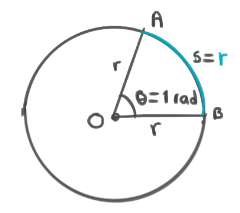
\includegraphics[width=4cm]{radian}
	\caption[Radian]{El radián.
		\begin{itemize}
			\item El arco $S$ tiene la misma medida que $\theta$ en grados
			\item El arco $S$ el unidades líneales mide $r$ (el radio).
		\end{itemize}
	}
	\labfig{radian}
\end{figure}

La unidad llamada radián se identifica a través del símbolo \textit{rad}

De la definición anterior debemos recordar siempre dos cosas:
\begin{itemize}
	\item \textbf{1 rad}\sidenote{Se lee como: ``un radián''} equivale a 
	$57.29^\circ$ \sidenote{No es necesario aprenderse este valor ya que para 
	calcularlo basta con recordar que el perímetro de la circunferencia es 
	$\boldsymbol{2r\pi}$. Y posteriormente realizar una sencilla regla de tres.}
	\item \fbox{ $\boldsymbol{\pi}$ \textbf{rad} equivale a $180^\circ$ }
\end{itemize}

\subsubsection{Conversión de grados a radianes y viceversa}
Los radianes y los grados tiene su equivalencia. De este modo, es posible medir 
los ángulos en grados o radianes según nos convenga. Para ello basta con un 
sencilla regla de tres, como se muestra a continuación.

\begin{example}
	Si queremos convertir $45^\circ$ a radianes.
	\begin{equation*}
	\begin{split}
		180^\circ &= \pi\; rad \\
		45^\circ &=  \boldsymbol{x}\\
		\Rightarrow x &= \dfrac{(45^\circ) (\pi\; rad)}{180^\circ}\\
		\therefore \boxed{ x = \dfrac{\pi}{4}\; rad }
	\end{split}
\end{equation*}
\end{example}

También se puede utilizar la regla de tres para convertir de radianes a grados.

\begin{example}
Convertir $\dfrac{\pi}{9}\; rad$ a grados.
\begin{equation*}
	\begin{split}
		180^\circ &= \pi\; rad \\
		\boldsymbol{x} &= \dfrac{\pi}{9}\; rad \\
		\Rightarrow x &= \dfrac{(180^\circ)
			\left(\dfrac{\pi}{9}\; rad \right)}{\pi\; rad} \\
		\therefore \boxed{ x = 20^\circ }
	\end{split}
\end{equation*}
\end{example}

Los dos tipos de conversiones se pueden realizar por medio de factores de 
conversión. Para ello tenemos las siguientes expresiones:

\begin{center}
	\renewcommand{\arraystretch}{1.2}
	\setlength{\tabcolsep}{20pt} % separacion de columnas
	\begin{tabular}{|c c |}
		\hline
		& \\
		\textbf{Grados a radianes} & \textbf{Radianes a grados}  \\ 
		$\alpha ^\circ \rightarrow\; rad$ & $rad \rightarrow \alpha ^\circ$ \\
		multiplicar por $\pmb{\dfrac{\pi}{180^\circ}}$ & 
		multiplicar por $\pmb{\dfrac{180^\circ}{\pi}}$ \\[5mm]		
		& \\
		\hline
	\end{tabular}
\end{center}

\begin{example}
	Convertir $75^\circ$ a radianes.
	$$75^\circ\left(\dfrac{\pi}{180^\circ} \right) = 
	\left( \dfrac{75^\circ}{180^\circ} \right) \pi\; rad = 
	\boxed{\left( \dfrac{5}{12}\right)\pi\; rad } $$
\end{example}

\begin{example}
	Convertir $\dfrac{7}{20} \pi\ rad$ a grados.
	$$\dfrac{7}{20} \pi\ rad \left(\dfrac{180^\circ}{\pi} \right) = 
		\left( \dfrac{7}{20} \right)(180^\circ) (\cancel{\pi\; rad})
		\left(\cancel{\dfrac{1}{\pi}}\right) = 
		7 \left(\dfrac{180^\circ}{20}\right) = 
		7 (9^\circ) = \boxed{63^\circ}
	$$
\end{example}

\begin{figure*}[hb!]
	\begin{kaoexercises}
		Convertir los siguientes ángulos a radianes
		\begin{multicols*}{4}
			\begin{enumerate}
				\setlength\itemsep{4mm}
				\item $210^\circ$
				\item $300^\circ$
				\item $225^\circ$
				\item $450^\circ$
				\item $72^\circ$
				\item $100^\circ$
				\item $330^\circ$
				\item $120^\circ$
				\item $135^\circ$
				\item $135^\circ$
			\end{enumerate}
		\end{multicols*}
		Convertir los siguientes ángulos a grados sexagesimales
		\begin{multicols*}{4}
			\begin{enumerate}
				\setlength\itemsep{4mm}
				\item $\dfrac{2}{3}\pi$
				\item $\dfrac{11}{6}\pi$
				\item $\dfrac{3}{4}\pi$
				\item $\dfrac{4}{3}\pi$
				\item $7 \pi$
				\item $\dfrac{1}{9} \pi$
				\item $\dfrac{13}{5} \pi$
				\item $\dfrac{1}{12} \pi$
				\item $\dfrac{5}{12} \pi$
				\item $\dfrac{9}{6} \pi$
			\end{enumerate}
		\end{multicols*}		
	\end{kaoexercises}
\end{figure*}

% Pseudo referencias
% https://oscarfruto.wixsite.com/angulos/sistema-ciclico
% http://maralboran.org/wikipedia/index.php/
%		Sistema_sexagesimal_de_medida_%281%C2%BA_ESO%29